\documentclass[../main.tex]{subfiles}
\begin{document}
    \chapter{Research Method}\label{chap:research_method}

    %This section will contain:
    %TODO: Explain the used method. %TODO research method
    %TODO: Hypothese/research questions %TODO research question

    \section{Introduction}
    $<<$ Todo: properly introduction of this chapter $>>$
    \\
    The analysis will be performed in this order:
    \begin{itemize}
        \item Resolve types
        \item Resolve sub type relations
        \item Extract facts from the source code
        \item Extract constraints from source code
        \item Solve the constraints
    \end{itemize}
    In the next step, annotations will be added to see how the results be like.
    
    \section{Research Question}
    The research question will be something like: \\
    \begin{quote}
        Will the use of phpdoc annotations produce better (to be defined) results for constraint based type inference?
    \end{quote}


    \section{Types}
    Explain here what I mean with a type...
    
    \begin{rascal}
\CAT{Keyword}{module} lang::php::m3::TypeSymbol

\CAT{Keyword}{data} TypeSymbol
  = any()
%  | array(\CAT{Keyword}{set}{}[TypeSymbol] itemTypes)
  | array()
  | \textbackslash{}bool()
  | class(\CAT{Keyword}{loc} decl)
  | float()
  | \textbackslash{}int()
  | object()
  | resource()
  | \textbackslash{}null()
  | string()
  | unset()
  ; 
    \end{rascal}
    
    \subsection{PHP types}
    PHP has a similar class inheritance structure and interface implementation as Java.
    The main difference is that in PHP all class are \texttt{public} and that inner classes are not allowed in PHP. 
    \\
    The basis types in PHP are integers, floats (similar to doubles and reals), booleans, strings, arrays, resources and null.
    When variables are initialised without a values, they are null. The recourse type is a special one which is not important for this research.
 
    \subsection{Subtypes}
    
    Explain something about subtypes here.

    %\blindtext %todo remove blind text
    
    \begin{figure}[H]
        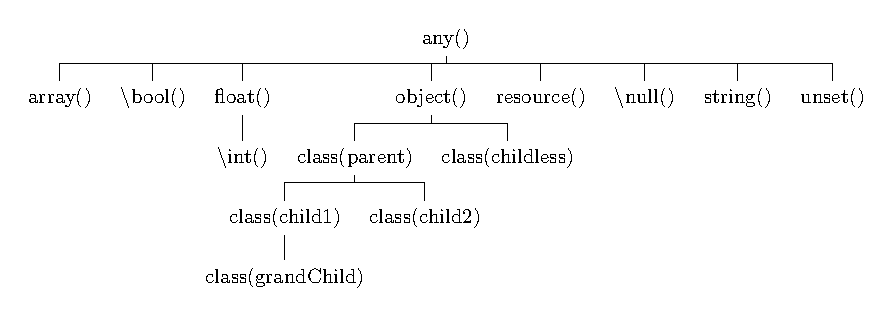
\includegraphics{Diagrams/Subtypes.pdf}
        \caption{Subtype hierarchy}
        \label{fig:subtypes}
    \end{figure}

    The subtype relation of class inheritance is a \gls{reflexive transitive closure} relation.
    A class extension of \textbf{\texttt{class A}} on \textbf{\texttt{class C}} will define \textbf{\texttt{class A}} as a subtype of \textbf{\texttt{class C}} in our analysis, as you can see in figure \ref{fig:subtypes}.
    If a class does not extend another class, it will implicitly extend the \gls{stdClass} class.
    You can see that this happens with \textbf{\texttt{class D}} in the example.
    The \textbf{\texttt{stdClass}} is represented as the type \textbf{\texttt{object()}} in our analysis.
    \\
    The basic PHP types also contain a subtype relation.
    Integers are subtypes of floats.
 
    % show three images next to each other
    \begin{figure}[H]
    \begin{subfigure}[b]{.33\textwidth}
      \begin{center}
      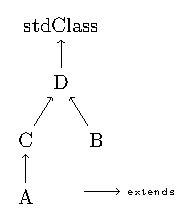
\includegraphics[scale=1]{Diagrams/Inheritance_example.pdf}
      \caption{Inheritance relation}
      \label{fig:subtype}
      \end{center}
    \end{subfigure}
    \begin{subfigure}[b]{.33\textwidth}
      \begin{center}
      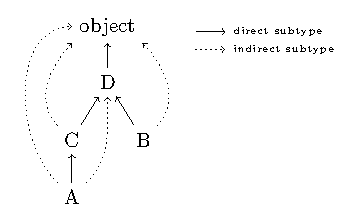
\includegraphics[scale=1]{Diagrams/Subtypes_example.pdf}
      \caption{Subtype relation}
      \label{subtype_tc}
      \end{center}
    \end{subfigure}
    \begin{subfigure}[b]{.33\textwidth}
      \begin{center}
      \lstinputlisting[xleftmargin=20pt,xrightmargin=20pt,language=PHP]{src/php/inheritance.php}
      \caption{Inheritance in PHP}
      \label{subtype_code}
      \end{center}
    \end{subfigure}
    \caption{Relation of subtypes among classes}
    \label{fig:subtypes}
    \end{figure}
    
    \section{Fact extraction}
    We can extract fact about classes, class-constants/fields/methods, functions, parameters.
    For these facts, we can use a relation, so we have a many-to-many relation.
    On the left size we will have the class, function or method. On the right side we have their attribute.
    \\
    A list of properties: (todo: rewrite this list into a `normal' section.) %todo rewrite this piece
    \begin{itemize}
        \item \textless{}loc classDecl, className(str name)\textgreater{}
        \item \textless{}loc classDecl, classMethod(str name, set[Modifier] modifiers)\textgreater{}
        \item \textless{}loc classDecl, classProperty(str name, set[Modifier] modifiers)\textgreater{}
        \item \textless{}loc classDecl, classConstant(str name, set[Modifier] modifiers)\textgreater{}
        \item \textless{}loc classDecl, classConstructorParameters(list[PhpParam] params)\textgreater{}
        
        \item \textless{}loc methodDecl, methodName(str name)\textgreater{}
        \item \textless{}loc methodDecl, methodParameters(list[PhpParam] params)\textgreater{}
        %\item \textless{}loc methodDecl, methodHasReturnStatements(bool)\textgreater{}
        
        \item \textless{}loc functionDecl, functionName(str name)\textgreater{}
        \item \textless{}loc functionDecl, functionParameters(list[PhpParam] params)\textgreater{}
    \end{itemize}
    
    In Rascal:
    \begin{rascal}
\CAT{Keyword}{alias} TypeFacts = \CAT{Keyword}{rel}{}[\CAT{Keyword}{loc} decl, Fact fact];

\CAT{Keyword}{data} Fact
    = className(\CAT{Keyword}{str} name) \CAT{Comment}{// may not be needed}
    | classMethod(\CAT{Keyword}{str} name, \CAT{Keyword}{set}{}[Modifier] modifiers)
    | classProperty(\CAT{Keyword}{str} name, \CAT{Keyword}{set}{}[Modifier] modifiers)
    | classConstant(\CAT{Keyword}{str} name, \CAT{Keyword}{set}{}[Modifier] modifiers)
    | classConstructorParameters(\CAT{Keyword}{list}{}[PhpParam] params)
    | methodName(\CAT{Keyword}{str} name) \CAT{Comment}{// may not be needed}
    | methodParameters(\CAT{Keyword}{list}{}[PhpParam] params)
    | functionName(\CAT{Keyword}{str} name) \CAT{Comment}{// may not be needed}
    | functionParameters(\CAT{Keyword}{list}{}[PhpParam] params)
    ;
    \end{rascal}
    
    \subsection{Type extraction}
    In order to define the subtype relations in class extensions, we will need to declare all existing class types.
    We can do this in rascal like is done in the example below:
    \begin{rascal}
\CAT{Keyword}{visit} (system) \{{}
    \CAT{Keyword}{case} c:class(\_{}, \_{}, \_{}, \_{}, \_{}): types += class(c@decl);
\}{}
    \end{rascal}
    Once all types are defined, we can add the subtype relation. We will need to have the subtype of \texttt{int()} and \texttt{float()} and the class extensions.
    You can see that in the code below:
    \begin{rascal}
\CAT{Keyword}{public} \CAT{Keyword}{rel}{}[TypeSymbol, TypeSymbol] getSubTypes(M3 m3, System system) 
\{{}
    \CAT{Keyword}{rel}{}[TypeSymbol, TypeSymbol] subtypes
        \CAT{Comment}{// add int() as subtype of float()}
        = \{{} \textless{}\textbackslash{}int(), float()\textgreater{} \}{} 
        \CAT{Comment}{// use the extends relation from M3}
        + \{{} \textless{}class(c), class(e)\textgreater{} | \textless{}c,e\textgreater{} \textless{}- m3@extends \}{}
        \CAT{Comment}{// add subtype of object for all classes which do not extends a class}
        + \{{} \textless{}class(c@decl), object()\textgreater{} | l \textless{}- system, /c:class(n,\_{},noName(),\_{},\_{}) \textless{}- system{}[l] \}{};
        
    \CAT{Comment}{// compute reflexive transitive closure and return the result }
    \CAT{Keyword}{return} subtypes*;        
\}{}
    \end{rascal}
  
    \subsection{Constraint extraction}
       
    Introduction is needed here... for now I will just list the types that I have found.
    Maybe this needs to be moved to a different chapter.
    \\
    \textbf{This is a list of items which are not supported (yet)}:

    \begin{itemize}
        
        \item References (in PHP they are symbol table aliases)
        \begin{itemize}
            \item on expression assignments :: $\$a \; = \; \&\$b$
            \item on functions :: function $\&f()$ $\{ \dots \}$
            \item on parameters :: function $f(\&\$a)$ $\{ \dots \}$             
        \end{itemize}

        \item Variable structures:
        \begin{itemize}
            \item \sout{Variable variables} :: $\$\$a;$
            \item \sout{Variable class instantiation} :: $new \; \$a;$
            \item \sout{Variable method or function calls} :: $\$a();$
        \end{itemize}

        \item List assign :: $list(\$a, \$b) = array("one", "two");$ (we can assume that the rhs is of type array, when the program is correct)
        
        \item \sout{Method or function parameters (including type hints)}
        \item \sout{Class structures, method calls}
        \item Class Constants
        
        \item \sout{The global statement} (should be resolved by the usage relation from M3)
        
        \item \sout{Casts of expressions}
        
        \item \sout{Predefined variables} (\$this, self, parent, static)

        \item \sout{Eval} (will not be supported)        
        \item \sout{Closures} (not used much in production code)
        \item \sout{Traits} (not used much in production code)
        \item \sout{Callable} (introduced in 5.4 as typehint, not used much in production code)
        
        \item Foreach(\$a as ... (=> ...)) => \$a is an array or an object;
        \item \sout{return; => return type is null} (is added to the situation when there are no return statements)
        \item add predefined globals (and their type: \$[GLOBALS, \_SERVER, \_GET, \_POST, \_REQUEST, \_COOKIE, \_ENV, \_SESSION, php\_errormsg] (all in global scope))
        \item add magic constants: \_\_[DIR, FILE, LINE, NAMESPACE, FUNCTION, CLASS, METHOD]\_\_
        \item predefined constants: TRUE(b), FALSE(b), NAN(f), INF(f), NULL(n), STDIN(r), STDOUT(r), STDERR(r) 
        \item define("name", value) mixed with constants (?out of scope?)
        \item \sout{keywords: self, parent, static in a class} (is included in method and property calls

        
        
    \end{itemize}

    \hrulefill
    
    \textbf{Legend} \\
    \begin{table}[H]
        \begin{tabular}{ c c l c c l }
            $=$     & = & Equal to (type) &
            $C$     & = & A class \\
            $<:$    & = & Is subTypeOf &
            $\rightarrow c$     & = & A class constant \\
            $E_k$   & = & An expression &
            $\rightarrow p$     & = & A class property \\
            $[E_k]$ & = & Type of some expression &
            $\rightarrow m$     & = & A class method \\
            $f$     & = & A function &
            $[m]$   & = & (Return) type of a method call \\
            $[f]$   & = & (Return) type of a function &
            $(A_n)$ & = & The n'th actual argument \\
            $::c$   & = & Static property fetch &
            $(P_n)$ & = & The n'th formal parameter \\
            $::m$   & = & Static method call &
            $th$    & = & Type hint \\
            $::p$   & = & Static property fetch &
            $v$     & = & Default value \\
            Mfs     & = & Modifiers &
            $\Gamma$ & = & Whole program 
            
            
        \end{tabular}
        \caption{Constraint legend}
        \label{table:constraintLegend}
    \end{table}
    
    \subsubsection{Expressions}
    Normal assignment:
    \begin{prooftree}
        \AxiomC{$E_1 = E_2$}
        \UnaryInfC{$[E_2]<:[E_1]$}
    \end{prooftree}
    \lstinputlisting[language=PHP,label=assignment1,caption=Assignment]{src/php/assignment1.php}
    \hrulefill

    Ternary:
    \begin{prooftree}
        \AxiomC{$E_1 \; ? \; E_2 : E_3 $}
        \UnaryInfC{$[E_1?E_2:E_3] = [E_3] \lor [E_4]$}
    \end{prooftree}
    \lstinputlisting[language=PHP,label=ternary,caption=Ternary]{src/php/ternary.php}
    \hrulefill

    Assignments with operators (1)
    \begin{prooftree}
        \AxiomC{
        ($E_1$ $\&=$ $E_2$) $\lor$
        ($E_1$ $\vert=$ $E_2$) $\lor$
        $E_1$ \^{}= $E_2$) $\lor$
        ($E_1$ $<<=$ $E_2$) $\lor$
        ($E_1$ $>>=$ $E_2$) $\lor$
        ($E_1$ $\%=$ $E_2$)
        }
        \UnaryInfC{$[E_1] = int()$}
    \end{prooftree}
    \lstinputlisting[language=PHP,label=assignment2,caption=Assignments with operators resulting in ints]{src/php/assignment2.php}
    \hrulefill

    Assignments with operators (2):
    \begin{prooftree}
        \AxiomC{$E_1$ .= $E_2$}
        \UnaryInfC{$[E_1] = string()$}
    \end{prooftree}    
    \lstinputlisting[language=PHP,label=assignment3,caption=Assignments with string concat operator]{src/php/assignment3.php}    
    \hrulefill
    
    Assignments with operators (3):
    \begin{prooftree}
        \AxiomC{
        ($E_1$ $/= E_2$) $\lor$
        ($E_1 -= E_2$)
        }
        \UnaryInfC{$[E_1] = int()$}
    \end{prooftree}    
    \lstinputlisting[language=PHP,label=assignment4,caption=Assignments with operators]{src/php/assignment4.php}
    \hrulefill

    Assignment with operators (4):            
    \begin{prooftree}
        \AxiomC{
        ($E_1$ *= $E_2$) $\lor$
        ($E_1$ += $E_2$)
        }
        \UnaryInfC{$[E_1] <: int()$}
    \end{prooftree}    
    \lstinputlisting[language=PHP,label=assignment5,caption=Assignments with operators]{src/php/assignment5.php}
    \hrulefill

    Comparison operators:    
    \begin{prooftree}
        \AxiomC{
        ($E_1$ $==$ $E_2$) $\lor$
        ($E_1$ $===$ $E_2$) $\lor$
        ($E_1$ $!=$ $E_2$) $\lor$
        ($E_1$ $<>$ $E_2$) $\lor$
        ($E_1$ $!==$ $E_2$)
        $\subseteq E$
        }
        \UnaryInfC{$[E] = bool()$}
    \end{prooftree}    
    \begin{prooftree}
        \AxiomC{
        ($E_1$ $<$ $E_2$) $\lor$
        ($E_1$ $>$ $E_2$) $\lor$
        ($E_1$ $<=$ $E_2$) $\lor$
        ($E_1$ $>=$ $E_2$)
        $\subseteq E$
        }
        \UnaryInfC{$[E] = bool()$}
    \end{prooftree}    
    \lstinputlisting[language=PHP,label=comparisonOperators.php,caption=Comparison operators]{src/php/comparisonOperators.php}
    \hrulefill
    
    Array declaration:
    \begin{prooftree}
        \AxiomC{$E'$, where $E'$ is an array declaration}
        \UnaryInfC{$[E'] = array()$}
    \end{prooftree} 
    \lstinputlisting[language=PHP,label=array,caption=Array declaration]{src/php/array.php}
    \hrulefill

    Array value fetch:
    \begin{prooftree}
        \AxiomC{$E_1[E_2]$ $\land$ $E_1 == string()$, where $E_1$ is an array}
        \UnaryInfC{$[E_1[E_2]] = string()$}
    \end{prooftree} 
    \begin{prooftree}
        \AxiomC{$E_1[E_2]$ $\land$ $E_1 == array()$, where $E_1$ is an array}
        \UnaryInfC{$[E_1[E_2]] = mixed()$}
    \end{prooftree} 
    \begin{prooftree}
        \AxiomC{$E_1[E_2]$ $\land$ $(E_1 == string()$ $\lor$ $E_1 == array())$, where $E_1$ is an array}
        \UnaryInfC{$[E_1[E_2]] = null()$}
    \end{prooftree} 
    \lstinputlisting[language=PHP,label=arrayAccess,caption=Array value fetch]{src/php/arrayAccess.php}
    \hrulefill
    
    \subsubsection{Scalars}
    Scalars:
    \begin{prooftree}
        \AxiomC{$E, E$ is a string*}
        \UnaryInfC{$[E] = string()$}
    \end{prooftree}
    * string can be single- or double- quoted, or be heredoc or nowdoc. (see below)
    \begin{prooftree}
        \AxiomC{$E, E$ is a float}
        \UnaryInfC{$[E] = float()$}
    \end{prooftree}
    \begin{prooftree}
        \AxiomC{$E, E$ is a integer}
        \UnaryInfC{$[E] = int()$}
    \end{prooftree}
    \lstinputlisting[language=PHP,label=scalar,caption=Scalars]{src/php/scalar.php}
    \hrulefill
    
    Encapsulated strings:
    \begin{prooftree}
        \AxiomC{$E, E$ is an encapsed string*}
        \UnaryInfC{$[E] = string()$}
    \end{prooftree}
    * When a string contains expression(/variables), it is processed as encapsed.
    \lstinputlisting[language=PHP,label=encapsed,caption=Encapsulated strings]{src/php/encapsed.php}
    \hrulefill
    
    \subsubsection{Casts}
    Casts:
    \begin{prooftree}
        \AxiomC{$(array)E_1$}
        \UnaryInfC{$[(cast)E_1] = array()$}
    \end{prooftree}
    \begin{prooftree}
        \AxiomC{$(bool)E_1$ $\lor$ $(boolean)E_1$}
        \UnaryInfC{$[(cast)E_1] = bool()$}
    \end{prooftree}
    \begin{prooftree}
        \AxiomC{$(float)E_1$ $\lor$ $(double)E_1$ $\lor$ $(real)E_1$}
        \UnaryInfC{$[(cast)E_1] = float()$}
    \end{prooftree}    
    \begin{prooftree}
        \AxiomC{$(int)E_1$ $\lor$ $(integer)E_1$}
        \UnaryInfC{$[(cast)E_1] = int()$}
    \end{prooftree}
    \begin{prooftree}
        \AxiomC{$(object)E_1$}
        \UnaryInfC{$[(cast)E_1] = object()$}
    \end{prooftree}
    \begin{prooftree}
        \AxiomC{$(unset)E_1$}
        \UnaryInfC{$[(cast)E_1] = null()$}
    \end{prooftree}
    \lstinputlisting[language=PHP,label=casts,caption=Casts]{src/php/casts.php}
    \hrulefill
            
    \subsubsection{Clone}
    Clone:
    \begin{prooftree}
        \AxiomC{$clone(E_1)$}
        \UnaryInfC{$[clone(E_1)] = object()$, $[E_1] = object()$}
    \end{prooftree}
    \lstinputlisting[language=PHP,label=clone,caption=Clone]{src/php/clone.php}
    \hrulefill
    
    \subsubsection{Class}
    Class instantiation (1) match class name:
    \begin{prooftree}
        \AxiomC{$new \; C$\textquotesingle{}() $\subseteq \Gamma$}
        \AxiomC{$class \; C$ ${ \dots }$ $\subseteq \Gamma$}
        \BinaryInfC{$[new \; C$\textquotesingle{}$] = C, \; C.name == C$\textquotesingle{}$.name$}
    \end{prooftree}
    \lstinputlisting[language=PHP,label=instantiation1,caption=Class instantiation]{src/php/instantiation1.php}
    \hrulefill

    Class instantiation (2):    
    \begin{prooftree}
        \AxiomC{
        $new \; E_1$
        $\subseteq \Gamma$
        }
        \UnaryInfC{$[new \; E_1]$ = object()}
    \end{prooftree}
    \lstinputlisting[language=PHP,label=instantiation2,caption=Class instantiation of an expression]{src/php/instantiation2.php}
    \hrulefill
    
    Special keywords:
    \begin{prooftree}
        \AxiomC{$\$ this \subseteq C$}
        \UnaryInfC{$[\$ this]$ = class(C)}
    \end{prooftree}
    \begin{prooftree}
        \AxiomC{$self \subseteq C$}
        \UnaryInfC{$[self]$ = class(C)}
    \end{prooftree}
    \begin{prooftree}
        \AxiomC{$parent \subseteq C$}
        \UnaryInfC{$[parent]$ = class(C.parent)}
    \end{prooftree}
    \begin{prooftree}
        \AxiomC{$static \subseteq C$}
        \UnaryInfC{$[static]$ = class(C$\textbar$C.parents)}
    \end{prooftree}
    
    Class method:
    \lstinputlisting[language=PHP,label=keywords,caption=Special keywords \texttt{\$this}]{src/php/keywords.php}
    \hrulefill
    
    Class property fetch* (1): \\
    \footnotesize{* Possible add fact that the field E is declared in class C, when it is on the left side of an assignment.}
    \begin{prooftree}
        \AxiomC{$\$this\rightarrow E_1 \subseteq C_1$}
        \UnaryInfC{$[E_1]$ = $C_1$.hasProperty($E_1$.name, static $\notin$ Mfs) $\lor$} \noLine
        \UnaryInfC{$[E_1]$ = $C_1$.parent.hasProperty($E_1$.name, public$\textbar$protected $\in$ Mfs $\land$ static $\notin$ Mfs) $\lor$} \noLine
        \UnaryInfC{$[E_1]$ = $C_1$[.parent].hasMethod("\_\_get")}
    \end{prooftree}
    \begin{prooftree}
        \AxiomC{$self :: E_1 \subseteq C_1$}
        \UnaryInfC{$[E_1]$ = $C_1$.hasProperty($E_1$.name, static $\in$ Mfs)}
    \end{prooftree}
    \begin{prooftree}
        \AxiomC{$parent :: E_1 \subseteq m$}
        \UnaryInfC{$[E_1]$ = C.parent.hasProperty($E_1$.name, static $\in$ Mfs )}
    \end{prooftree}
    \begin{prooftree}
        \AxiomC{$E_1\rightarrow E_2 \subseteq C_1$*}
        \UnaryInfC{$[E_1]$ = $C_1$.hasProperty($E_2$.name, static $\notin$ Mfs) $\lor$} \noLine
        \UnaryInfC{$[E_1]$ = $C_1$.parent.hasProperty($E_2$.name, public$\textbar$protected $\in$ Mfs $\land$ static $\notin$ Mfs) $\lor$} \noLine
        \UnaryInfC{$[E_1]$ = $C$.hasProperty($E_2$.name, public $\in$ Mfs $\land$ static $\notin$ Mfs)}
    \end{prooftree}
    \footnotesize{*The same goes for static property fetches, except for the `static $\notin$ Mfs' part: `static $\in$ Mfs'.}
    \begin{prooftree}
        \AxiomC{$E_1\rightarrow E_2 \not\subseteq C \subseteq \Gamma$*}
        \UnaryInfC{$[E_1]$ = C.hasProperty($E_2$.name, public $\in$ Mfs $\land$ static $\notin$ Mfs)}
    \end{prooftree}
    \footnotesize{*Property fetch outside a class scope, also for static properties.}
    \lstinputlisting[language=PHP,label=property1,caption=Class property]{src/php/property1.php}
    \hrulefill
    
    Class property (2) variable:
    \begin{prooftree}
        \AxiomC{$E_1\rightarrow E_2$, $E_2$ is an expression}
        \UnaryInfC{$[E_1]$ = object()}
    \end{prooftree}
    \lstinputlisting[language=PHP,label=property2,caption=Class property variable]{src/php/property2.php}
    \hrulefill
  
    Class method call (1): 
    \begin{prooftree}
        \AxiomC{$\$this\rightarrow E_1 \subseteq C_1$}
        \UnaryInfC{$[E_1]$ = $C_1$.hasMethod($E_1$.name, static $\notin$ Mfs) $\lor$} \noLine
        \UnaryInfC{$[E_1]$ = $C_1$.parent.hasMethod($E_1$.name, public$\textbar$protected $\in$ Mfs $\land$ static $\notin$ Mfs) $\lor$} \noLine
        \UnaryInfC{$[E_1]$ = $C_1$[.parent].hasMethod("\_\_call")}
    \end{prooftree}
    \begin{prooftree}
        \AxiomC{$self :: E_1 \subseteq C_1$}
        \UnaryInfC{$[E_1]$ = $C_1$.hasMethod($E_1$.name, static $\in$ Mfs) $\lor$} \noLine
        \UnaryInfC{$[E_1]$ = $C_1$.parent.hasMethod($E_1$.name, public$\textbar$protected $\in$ Mfs $\land$ static $\in$ Mfs) $\lor$} \noLine
        \UnaryInfC{$[E_1]$ = $C_1$.hasMethod("\_\_callStatic")}
    \end{prooftree}
    \begin{prooftree}
        \AxiomC{$parent :: E_1 \subseteq C_1$}
        \UnaryInfC{$[E_1]$ = $C_1$.parent.hasMethod($E_1$.name, public$\textbar$protected $\in$ Mfs) $\lor$} \noLine
        \UnaryInfC{$[E_1]$ = $C_1$.parent.hasMethod("\_\_callStatic")}
    \end{prooftree}
    \begin{prooftree}
        \AxiomC{$E_1\rightarrow E_2 \subseteq C_1$*}
        \UnaryInfC{$[E_1]$ = $C_1$.hasMethod($E_2$.name, static $\notin$ Mfs) $\lor$} \noLine
        \UnaryInfC{$[E_1]$ = $C_1$.parent.hasMethod($E_2$.name, public$\textbar$protected $\in$ Mfs $\land$ static $\notin$ Mfs) $\lor$} \noLine
        \UnaryInfC{$[E_1]$ = $C$.hasMethod($E_2$.name, public $\in$ Mfs $\land$ static $\notin$ Mfs)}
    \end{prooftree}
    \footnotesize{*The same goes for static method calls, except for the `static $\notin$ Mfs' part: `static $\in$ Mfs'.}
    \begin{prooftree}
        \AxiomC{$E_1\rightarrow E_2 \not\subseteq C \subseteq \Gamma$*}
        \UnaryInfC{$[E_1]$ = C.hasMethod($E_2$.name, public $\in$ Mfs $\land$ static $\notin$ Mfs)}
    \end{prooftree}
    \footnotesize{*method call outside a class scope, also for static methods.}
    \lstinputlisting[language=PHP,label=methodCall1,caption=Class method call]{src/php/methodCall1.php}
    \hrulefill

    Method calls (2) variable
    \begin{prooftree}
        \AxiomC{$E_1$ $\rightarrow$ $E_2$(), $E_2$ is an expression}
        \UnaryInfC{$[E_1]$ = object() }
    \end{prooftree}
    \lstinputlisting[language=PHP,label=methodCall2,caption=Variable method call]{src/php/methodCall2.php}
    \hrulefill

    Class constants*
    \footnotesize{*This on class constants sections needs to be reviewed...}
    \begin{prooftree}
        \AxiomC{self::$c_1$ $\subseteq$ $\Gamma$}
        \UnaryInfC{$[$self::$c_1]$ = $C_1$.hasConstant($E_2$.name) $\lor$} \noLine
        \UnaryInfC{$[$self::$c_1]$ = $C_1$.parent.hasConstant($E_2$.name, public$\textbar$protected $\in$ Mfs)}
    \end{prooftree}
    \begin{prooftree}
        \AxiomC{parent::$c_1$ $\subseteq$ $\Gamma$}
        \UnaryInfC{$[$self::$c_1]$ = $C_1$.parent.hasConstant($E_2$.name, public$\textbar$protected $\in$ Mfs)}
    \end{prooftree}
    \begin{prooftree}
        \AxiomC{$E_1$::$c_1$ $\subseteq$ $\Gamma$}
        \UnaryInfC{$[E_1]$ = object() }
    \end{prooftree}
    \lstinputlisting[language=PHP,label=classConstants,caption=Class constants]{src/php/classConstants.php}
    \hrulefill
    
    \subsubsection{Parameters}
    Parameters in class instantiation*:
    \begin{prooftree}
        \AxiomC{$new \; C_1$ ($A_1$, $A_2$, $\dots$, $A_k$) $\subseteq \Gamma$} \noLine
        \UnaryInfC{$\$a \rightarrow m$() ($A_1$, $A_2$, $\dots$, $A_k$) $\subseteq \Gamma$} \noLine
        \UnaryInfC{$function_1$ ($A_1$, $A_2$, $\dots$, $A_k$) $\subseteq \Gamma$}
        \AxiomC{$class \; C$ ($th_1$ $P_1$, $P_2$ = $v$, $\dots$, $P_k$) $\subseteq \Gamma$} \noLine
        \UnaryInfC{public function $m$() ($th_1$ $P_1$, $P_2$ = $v$, $\dots$, $P_k$) $\subseteq \Gamma$} \noLine
        \UnaryInfC{function ($th_1$ $P_1$, $P_2$ = $v$, $\dots$, $P_k$) $\subseteq \Gamma$}
        \BinaryInfC{$[P_1]<:[A_1]$, $[A_1]<:[th_1]$, $[P_1]<:[th_1]$, hasRequiredParam($P_1$), hasRequiredParam($P_k$)}
    \end{prooftree}
    \footnotesize{*These parameters are just examples for what happens if they have typeHints ($th$), default values($v$) or none}
    \footnotesize{*The constructor can be found in the m3 model (@constructors(loc classDecl, loc constructorMethodDecl))}
    \lstinputlisting[language=PHP,label=parameter1,caption=Class instantiation with parameters]{src/php/parameter1.php}
    \hrulefill


    Type of a certain variable within some scope:
    \begin{prooftree}
        \AxiomC{$E, E', E'', E''' \dots \; etc$ $\subseteq f$}
        \AxiomC{$E$ is a variable}
        \BinaryInfC{$[E] = [E] \lor [E'] \lor [E''] \lor [E'''] \dots \; etc$}
    \end{prooftree}    
    \lstinputlisting[language=PHP,label=function1,caption=Type of variable within their scope; this applies to global- class- function- and method- scope]{src/php/function1.php}
    \hrulefill
    
    Return type of function or method (1):
    \begin{prooftree}
        \AxiomC{return $\not \subseteq f$ $\lor$ return; $\subseteq f$}
        \UnaryInfC{$[f] = null()$}
    \end{prooftree}    
    \lstinputlisting[language=PHP,label=return1,caption=No return statements in function or method]{src/php/return1.php}
    \hrulefill
    
    Return type of function or method (2):
    \begin{prooftree}
        \AxiomC{
        (return $E_1$) $\lor$
        (return $E_2$) $\lor$
        $\cdots$ $\lor$
        (return $E_k$)
        $\subseteq f$
        }
        \UnaryInfC{$[f] <: [E_1] \lor [E_2] \lor \cdots \lor [E_k]$}
    \end{prooftree}    
    \lstinputlisting[language=PHP,label=return2,caption=Return of a function or method; every exit path ends with a return statement]{src/php/return2.php}
    \hrulefill
    
    Return type of function or method (3):    
    \begin{prooftree}
        \AxiomC{
        (return $E_1$) $\lor$
        (return $E_2$) $\lor$
        $\cdots$ $\lor$
        (return $E_k$) $\lor$
        ($\neg$ return)
        $\subseteq f$
        }
        \UnaryInfC{$[f] <: [E_1] \lor [E_2] \lor \cdots \lor [E_k] \lor null() $}
    \end{prooftree}    
    \lstinputlisting[language=PHP,label=return3,caption=Return with possible no return value]{src/php/return3.php}
    \hrulefill
        
    Function call:
    \begin{prooftree}
        \AxiomC{
        $f()$
        $\subseteq \Gamma$
        }
        \UnaryInfC{$[f()] <:$ return of $[f]$}
    \end{prooftree}    
    \lstinputlisting[language=PHP,label=functionCall1,caption=Functional call]{src/php/functionCall1.php}
    \hrulefill
    
    Variable function call:
    \begin{prooftree}
        \AxiomC{
        $E_1()$ $\subseteq \Gamma$
        }
        \UnaryInfC{$[E_1()] = mixed()$}
    \end{prooftree}    
    \lstinputlisting[language=PHP,label=functionCall2,caption=Variable function call]{src/php/functionCall2.php}
    \hrulefill
    
    How to resolve expressions:
    \begin{itemize}
        \item Find all expressions which are defined above and annotate them with @type.
        \item Annotate the rest of the expressions with @type = any();
    \end{itemize}
    
    \section{Annotations}
    Explain how the annotations are added to the constraints.
    %\Blindtext
    
    \section{Constraint solving}
    Explain what will be done to solve the constraints.
    \\
    %\Blindtext
    
    \section{Case Study}
    Explain how the case study is performed. (maybe move this section to a separate chapter)
    \\
    %\Blindtext

\end{document}
